\chapter{The Uniscale Frangi Filter} \label{ch:unifrangi}

	We now seek to harness the ideas of this section to the task at hand: identifying curvilinear content within images.
\section{The Frangi Filter: Uniscale} \label{sec:frangi}

The Frangi filter, first described by Alejandro Frangi et al. in \cite{frangi-paper} is a widely used  Hessian-based filter
within image processing. Hessian-based filters make use of the
logical ``proximity'' of the Hessian to notions of curvature of surfaces,
as developed in \cref{sec:differential-geometry}. 
Several such Hessian-based filters exist--see \cite{sato-filter} and \cite{lorenz-filter}, as well as a comparison given in \cite{olabarriaga-hessian-comparison}. These filters use information about the principal curvatures, approximated as eigenvalues of the Hessian) at each point in the image
to identify regions of significant curvature within an image.

\vcleanup{move to next section? or cover any necessary math here}

Frangi's filter was orignally developed for vascular segmentation in images such as MRIs and it excels in that context.

The procedure for a single scale in a 2D image is as follows:
Let $\lambda_1, \lambda_2$ be the two eigenvalues of the Hessian of the image at point $(x, y)$,
ordered such that $\abs{\lambda_1} \leq \abs{\lambda_2}$, and define the Frangi vesselness measure %at scale $\sigma$ as:
as:

\begin{equation} \label{eq:frangi-vesselness-measure}
\Vsigma(x_0,y_0) = \begin{cases}
0 & \text{if} \quad \lambda_2 > 0 \\
\exp\left\{-\frac{A^2}{2\beta^2}\right\}
\left(1 - \exp\left\{-\frac{S^2}{2c^2}\right\}\right) & \text{otherwise}
\end{cases} \end{equation}
where
\begin{equation} \label{frangi-def-anisotropy-structureness}
A := \abs{\lambda_1 / \lambda_2}
\quad \textrm{and} \quad 
S := \sqrt{\lambda_1^2 + \lambda_2^2}
\end{equation}
and $\beta$ and $c$ are tuning parameters. Before we discuss appropriate values for $\beta$ and $c$, we first seek to highlight the significance of \cref{eq:frangi-vesselness-measure}, and in particular, the ratios defined in
\cref{frangi-def-anisotropy-structureness}. $A$ and $S$ are known as the anisotropy measure and structureness measure, respectively. Consequently, we'll refer to the two factors in \cref{eq:frangi-vesselness-measure} as the anisotropy factor and structureness factor, respectively. 

\subsection{Anisotropy Measure} \label{sec:frangi.anisotropy}
The anisotropy (or directionality) measure $A$ is simply the ratio of magnitudes of $\lambda_1$ and $\lambda_2$. Since at a ridge point of a tubular structure, we should have $\lambda_1 \approx 0$ and $\abs{\lambda_2} \gg \abs{\lambda_1}$,
a very small value of $A$ would be present at a ridge of a tubular structure.

\begin{figure} \centering
  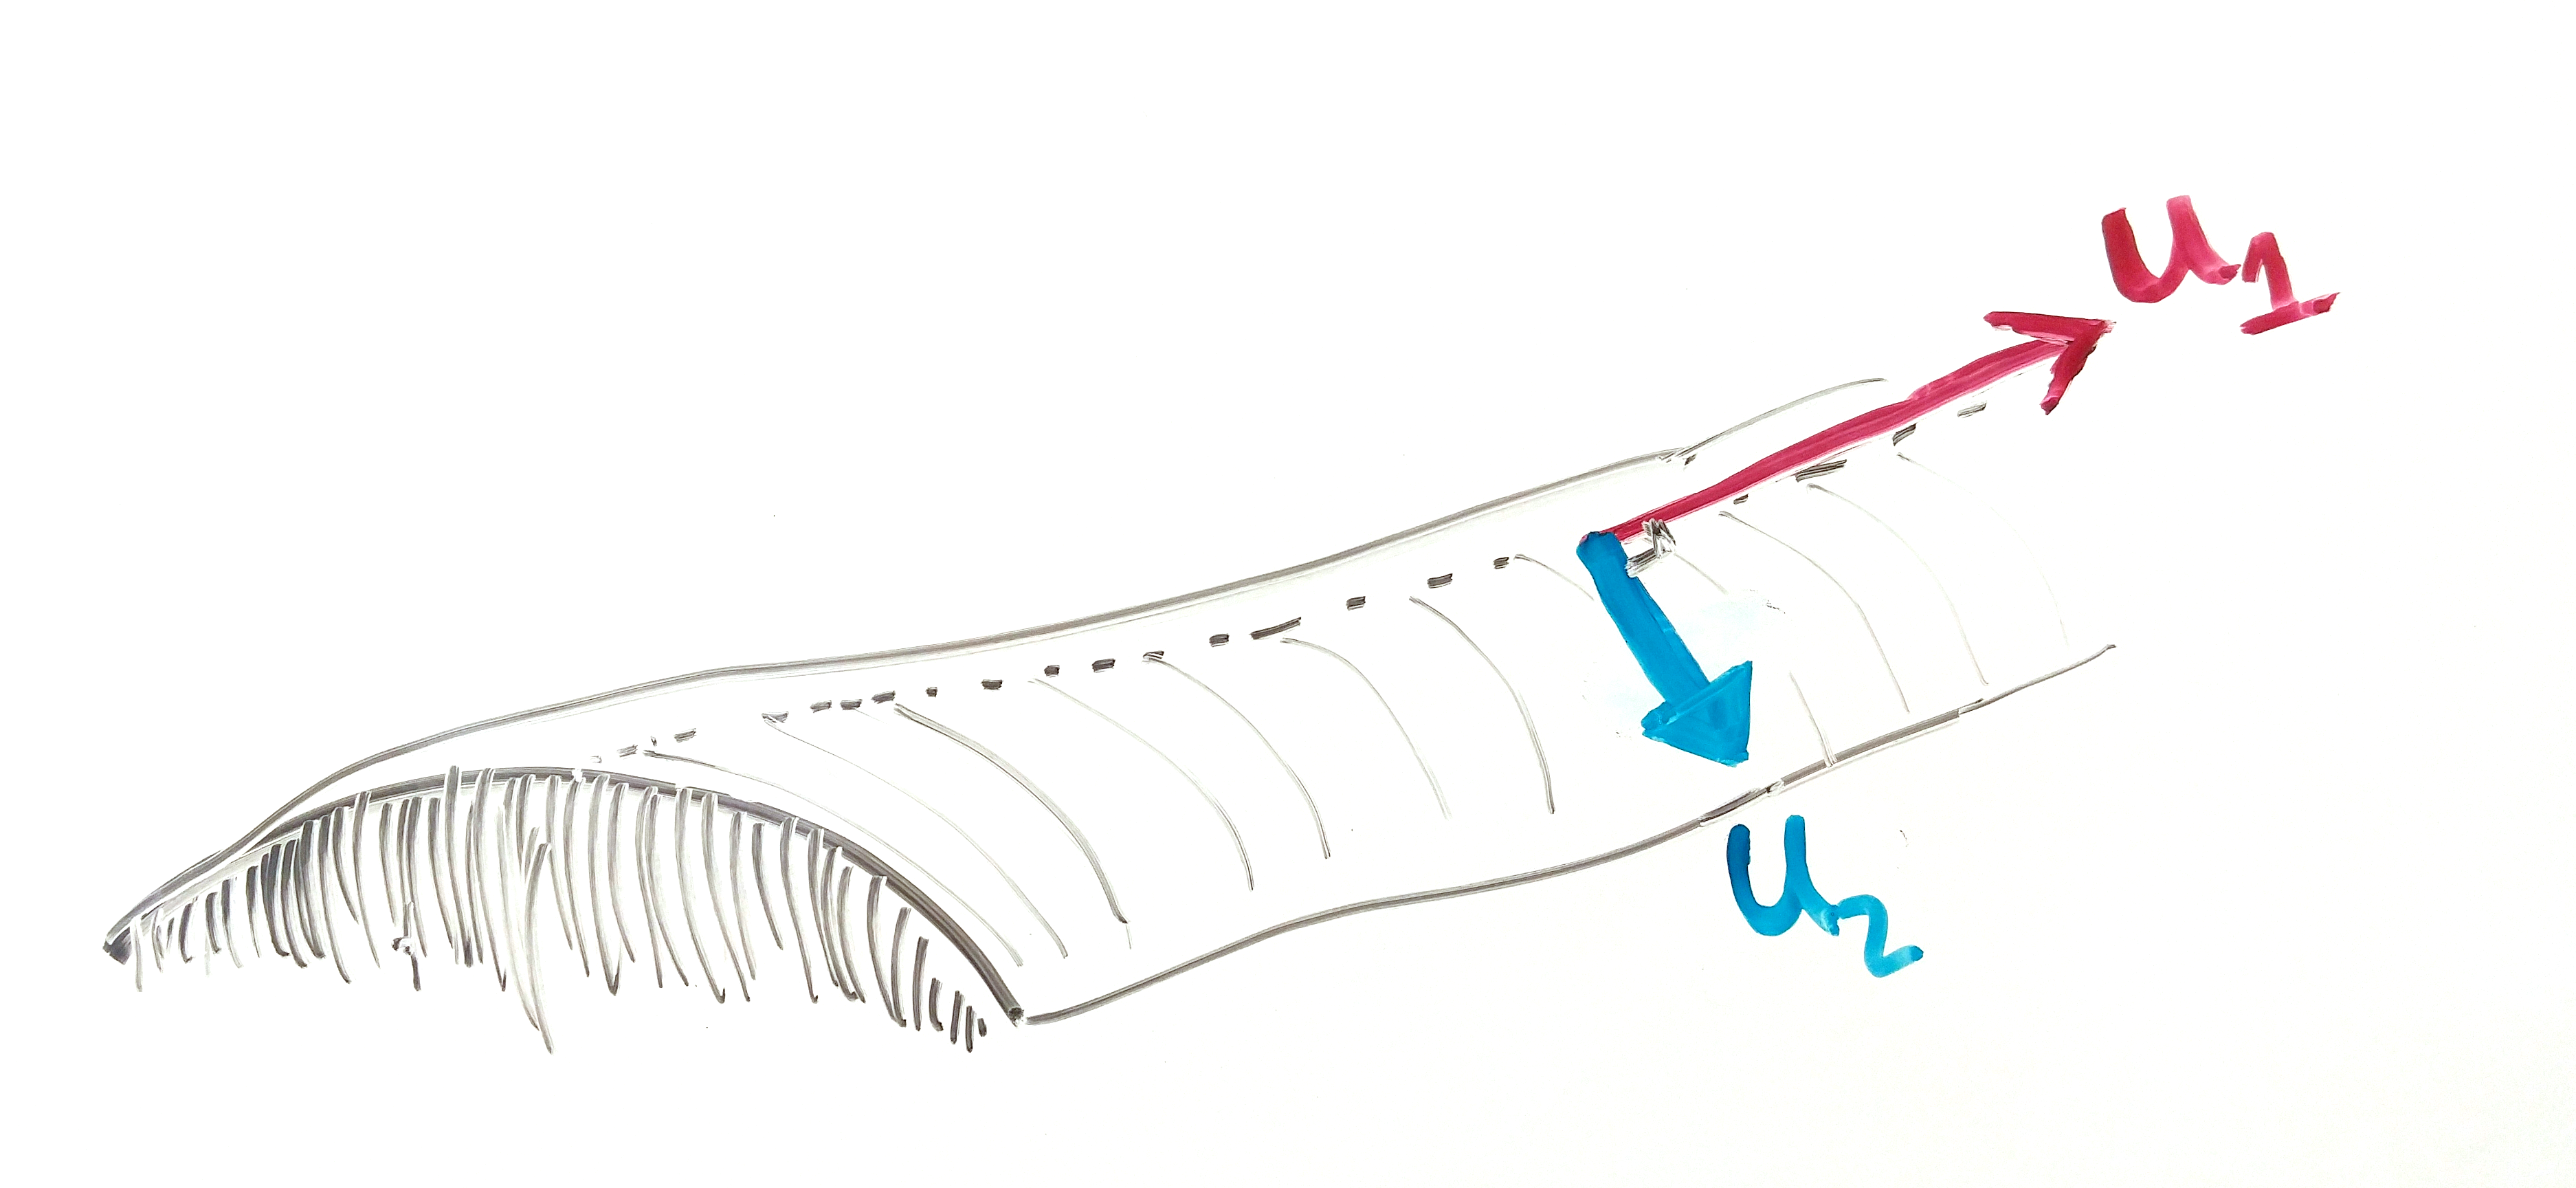
\includegraphics[width=0.8\linewidth]{expo_principal_curvatures}
  \caption{The principal eigenvectors at a ridge like structure} 
  \label{fig:expo-principal-curvatures}
\end{figure}

In \cref{fig:expo-principal-curvatures}, this situation is demonstrated. Here, $u_1, u_2$ form the orthogonal set of Hessian eigenvectors with corresponding eigenvalues $\lambda_1$ and $\lambda_2$. At such a ridgelike structure, we could predict the largest change in curvature to be straight down the ridge (in the direction of $u_2$), and the direction of least curvature to be directly along the ridge (in the direction  of $u_1$). $\lambda_1 \approx 0$ and $\lambda_2$ is large and negative.

Of course, if the the ridge is perfectly circular along its cross section (as was in \cref{sec:calculate-weinmap-of-a-ridge}, it is of course apparent that $\lambda_2$ would be the same value at any place along the ridge (not just at its crest \vcleanup{fix terminology}), and $\lambda_1$ would likewise be 0 at any such point.  One could also imagine a similar situation in which the dropoff from crest to bottom gets increasing steep. In such a case, $\lambda_2$ as a function of $x$ would in fact be largest nearest to the bottom. This thought experiment should dispel a na\"{i}ve misunderstanding of the power of a Frangi filter: a high anisotropy measure (and a large structureness measure \vcleanup{define structureness first}) will not in general identify the crests of a ridge-like structure--it only will highlight that such a pixel is on a ridge-like structure at all. Thus, the anisotropy measure will not necessarily be at a maximum at the crest of the ridge, but instead, somewhere along it.

Similiarly, the vessel we we wish to identify can not be reasonably expected to behave as perfectly as our toy example. There will likely be small aberrations in a ridgelike structure, such as small divots or depressions in an overall ridge-like structure. Of importance in our data set later ( \cref{sec:NCS-data-set}), there will be points where we seem to "lose" our ridgelike structure,
but this is simply due to an error in the sample.

Importantly, this formulation does not require $\lambda_1$ to be approximately zero, just that the curvature in the downward direction is much more significant than in the transverse direction.

Also the crest could be really flat (``hangar shaped''), in which case both are around zero. At the crest of the ridge, we would actually expect both $u_1$ and $u_2$ to be around 0, whereas a point somewhere between the crest and the ``foot'' of the ridge to contain the maximum $u_2$. We will fix this issue specificially by casting this as a multiscale problem in \cref{sec:frangi-multiscale}.

Two other ideas that could fix some other discrepancies mentioned above is to identify these ridges on their own, or also where the 'feet are'. We will discuss these ideas in \cref{sec:future-research-directions}.

\subsection{Structureness measure} \label{sec:frangi-structureness}

There is another concern with using the pure ratio $S:= \abs{\lambda_1 / \lambda_2}$ as an identifying feature of ridgelike structures apart from the ones listed above. We could have $\abs{\lambda_2} \gg \abs{\lambda_1}$ in a relative sense, but still have $\lambda_2 \approx 0$. As a rather extreme example, we should certainly wish to differentiate a point on the surface where $\lambda_2 \approx 10^{-5} $ and $\lambda_1 \approx 10^{-10}$ from another point where $\lambda_2 \approx 10000$ and $\lambda_2 = 0.1$.

A natural fix to differentiate these points is to introduce a ``structureness'' measure to insure that there is in fact significant curvilinear activity at the point in question. Frangi used $S:= \sqrt{(\lambda_1)^2 + (\lambda_2)^2}$, which is in fact the Frobenius norm of the Hessian matrix. Thus the Frangi filter should also prefer areas of
great curvilinear content in the image first of all.


\subsection{The Frangi vesselness measure}

Our goal then is to attach a numerical measure to each pixel in the image (at a particular scale $\sigma$) that is large when the anisotropy measure $A$ and the structureness measure $S$ is sufficiently large.

The form Frangi arrived at in \cref{eq:frangi-vesselness-measure} in which a factor of $\exp\{...\}$ and $(1 - \exp\{...\})$ are multiplied together are simply to ensure that the final vesselness measure $V$ is largest when $A$ is small and $S$ is large enough, with rapid decay in other situations.

Frangi further strengthened the filter by adding an additional case to in \cref{eq:frangi-vesselness-measure}, ensuring that $\lambda_2$ is not positive. If we are indeed at a curvilinear ridge, we need the second derivative of the surface in the maximal direction to be negative, which hasn't been accounted for as yet in our formulation of $A$ and $S$ -- we wish (for our purposes) to only identify when we are finding crests. $A$ will still be small and $S$ will still be large however if we identify a ``trough''.

The only perceivable difference is that the maximum normal curvature will be positive--we are at a local minimum in the direction of $u_2$. In situations where we wish to only identify ridges (as is the case here) we simply exclude any points where there is not a negative curvature in the maximal direction. Conversely, we could only seek to find valley, or local minima, as thus require $\lambda_2 > 0$, and set the vesselness measure to zero when $\lambda_2 < 0$.

\subsection{Choosing parameters $\beta$ and $c$}

The parameters $\beta$ and $c$ are meant to scale so that the peaks of the anisotropy factor $\exp\{\frac{-A^2}{2\beta^2}\}$ and the structureness factor $(1-\exp\{\frac{-S^2}{2c^2}\})$ coincide enough to be statistically significant at highly curvilinear structures, but rapidly decay in areas not associated with curvilinear content. What values of these parameters are appropriate is ultimately dependent on the context of the problem.

Frangi suggested for $c$ that half of (the Frobenius norm of the) Hessian matrix is appropriate, simply because the minimum value of $S$ is zero, and its maximum value is exactly the max Frobenius norm. With this in mind we would like to introduce the scaling factor
$\gamma$, so that $ c = \gamma S_{\max}$. This creates a minor annoyance though: although the anisotropy factor can certainly attain a value of 1, if $c$ is to take this ``appropriate'' value, the maximum value of the structureness factor is somewhat smaller than 1. In fact,
\begin{equation}
\begin{aligned}
\max\{\Vsigma\} &\le \max\left(
\exp\left\{\frac{-A^2}{2\beta^2}\right\}
\right)
\max\left(
\left(1 - \exp\left\{\frac{-S^2}{2(\gamma S_{\max})^2}\right\}\right)
\right) \\
&\le \max\left\{
\left(1 - \exp\left\{\frac{-S^2}{2(\gamma S_{\max})^2}\right\}\right)
\right\} \\
&= 
\left(1 - \exp\left\{\frac{-(S_{\max})^2}{2(\gamma S_{\max})^2}\right\}
\right)
= \left(1 - \exp\left\{\frac{-1}{2\gamma^2}\right\}
\right)
\end{aligned}
\end{equation}

Thus, when $\gamma$ takes the suggested value of $\gamma = 1/2$, the above calculation suggests that
the maximum theoretical value that the Frangi filter could attain at any scale is
$ \max \{ \Vsigma \} \le 1 - \exp\left\{ -1 \right\} \approx .8647$.
This (among other obvious reasons) certainly justifies Frangi's description of the vesselness measure as only ``probability-like.'' Still, we would like the filter's sensitivity to relative structureness to not have the effect of dampening the Filter as a whole, so we will introduce a rescaling factor $a_\gamma$, which is a explicit function of $\gamma$ that rescales $\Vsigma$ so that the structureness factor has a maximum output score of 1 regardless of choice of $\gamma$. Our final Frangi vesselness measure is thus

%    \begin{minipage}{\textwidth} \centering
\begin{gather} \label{eq:frangi-vesselness-measure-v1}
\Vsigma(x_0,y_0) = \begin{cases}
0 & \text{if} \quad \lambda_2 > 0 \\
a_\gamma \exp\left\{\frac{-A^2}{2\beta^2}\right\}
\left(1 - \exp\left\{\frac{-S^2}{2(\gamma S_{\max})^2}\right\}\right) & \text{otherwise}
\end{cases} \\
\shortintertext{where, as before,}
%\begin{equation} \label{frangi-def-anisotropy-structureness-v1}
A := \abs{\lambda_1 / \lambda_2}
\;,\;
S := \sqrt{\lambda_1^2 + \lambda_2^2}
\;\textrm{and}\;
a_\gamma = \left(1-\exp\left(\frac{-1}{2\gamma^2}\right)\right)^{-1} \notag\\
%\end{equation}
\shortintertext{and}
%\begin{equation*}
\abs{\lambda_1} \le \abs{\lambda_2}
\; \textrm{are eigenvalues of}\; \Hess_\sigma(\img(x_0, y_0)) \notag
%\end{equation*}
\end{gather}
%    \end{minipage}

For $\beta$, Frangi suggested an innocuous intermediate point, $\beta=1/2$ (and thus $2\beta^2 = 1/2$).
As we will show later, choosing the structureness parameter $\gamma$ is rather important for the context especially if the background (non-ridgelike structure) is significant and noisy. $\beta$ should be strengthened/relaxed depending on how ``flat'' the ridgelike structure is. We shall show empirically that contexts in which more 'bloblike' structures are known to be present than that for which the Frangi filter was originally designed, we will benefit from a smaller choice of $\beta$.

Considering as the anisotropy measure $\abs{\lambda_1 / \lambda_2} \in [0,1]$ (simply since $\abs{\lambda_1} \le \abs{\lambda_2}$), we can actually visualize how much the 
anisotropy factor varies depending on our choice of $\beta$, as seen in \cref{fig:anisotropy-parameter-demo}.

We can theoretically choose any values $0 < \beta, \gamma < \infty$ for the two parameters. Two particular limits are of theoretical interest:
as $\beta \to \infty$, the anisotropy factor tends to $1$, and as $\gamma \to 0$, the structureness factor tends to $1$, make the that measure entirely irrelevant. (Of course, in the limit that $\beta \to 0$ or $\gamma \to \infty$, their respective factors become 0, making the entire filter irrelevant). We will 
\begin{figure}
  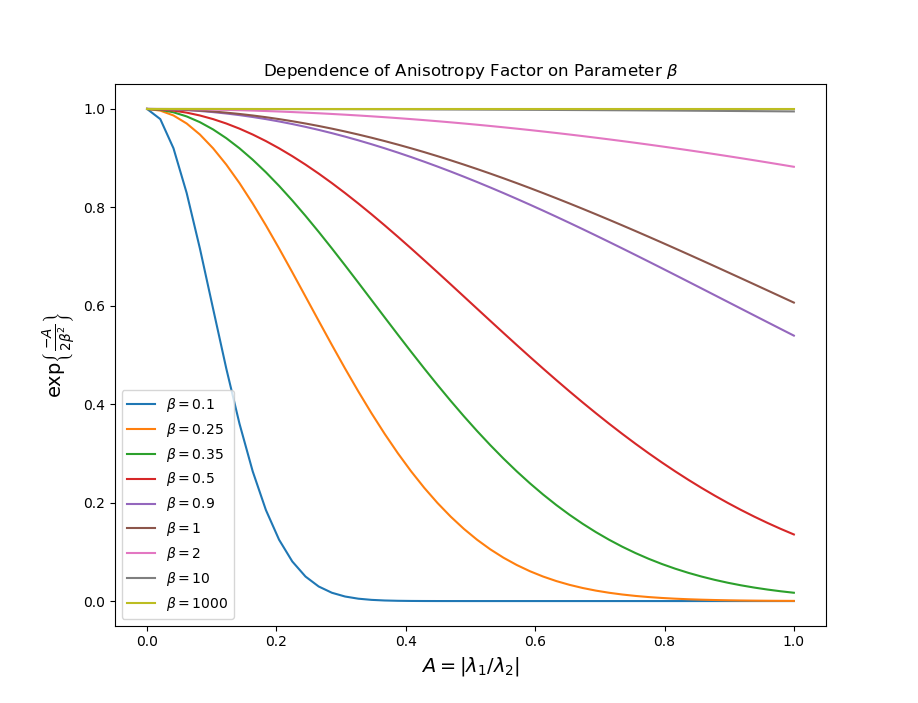
\includegraphics[width=\linewidth]{anisotropy_parameter_demo}
  \caption{Dependence of the Anisotropy Factor on its Parameter}
  \label{fig:anisotropy-parameter-demo}
\end{figure}

We make a similar presentation of the dependence of the structureness kernel on its parameter $\gamma$, as you can see in \cref{fig:structureness-parameter-demo}.
\begin{figure}
  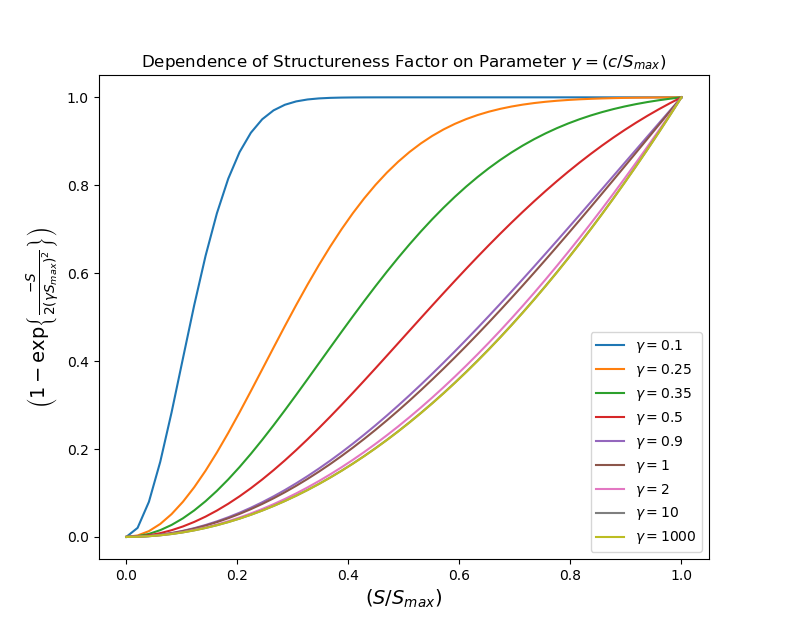
\includegraphics[width=\linewidth]{structureness_parameter_demo}
  \caption{Dependence of the Structureness Factor on its Parameter}
  \label{fig:structureness-parameter-demo}
\end{figure}

The ultimate choice of these parameters $\beta$ and $\gamma$ have the overall effect of tuning the selectivity of the Frangi filter itself.
In the figures in \cref{app:extra-figures}, we plot the Frangi vesselness measure itself as a function of $S$ and $A$ while sweeping through different choices of $\beta$ and $\gamma$. 


	We now take a quick tangent from our description of the Frangi filter to develop and justify our ``multiscale'' approach.